\documentclass{article}

\usepackage{graphicx}

\title{Making a State Machine}
\author{Joey Kilgore}

\begin{document}
\maketitle

\section{Overview}
In this project we will create a state machine that will allow us to give inputs and go from one state to another. The end goal will do the following

\begin{enumerate}
\item Read in a file containing the states and the transitions
\item Have the user enter what state they would like to start in
\item Have the user enter a transition and output the new state they are in
\item Repeat the previous step until the user enters ``EXIT''
\end{enumerate}

With this we will have to focus on utilizing data structures to improve our ability to solve a problem, and noting that there are multiple ways to store data that still solve this problem.

\section{Background}
\subsection{Alexa}
State machines (in this case more formally determinitistic finite automata) are useful in multiple facets of computer science and practical applications in real software. State machines become a good way to conceptualize how something works on a functional level. As an initial example we can look at a simplified diagram that gives a general idea of how states and transitions create a functional diagram.

From the Alexa diagram in Figure \ref{fig:alexa} we can pull out the following things which are useful notes in functionality.

\begin{itemize}
\item We cannot immediately ask for the temperature without being in the \textit{LISTENING} state
\item We cannot immediately ask another question without saying ``Hey Alexa'' again
\item The process loops forever
\item Information on \textbf{any} question asked can be reported back at the \textit{STOP LISTENING} state which all questions must eventually get to.
\end{itemize}

\begin{figure}[!h]
\centering
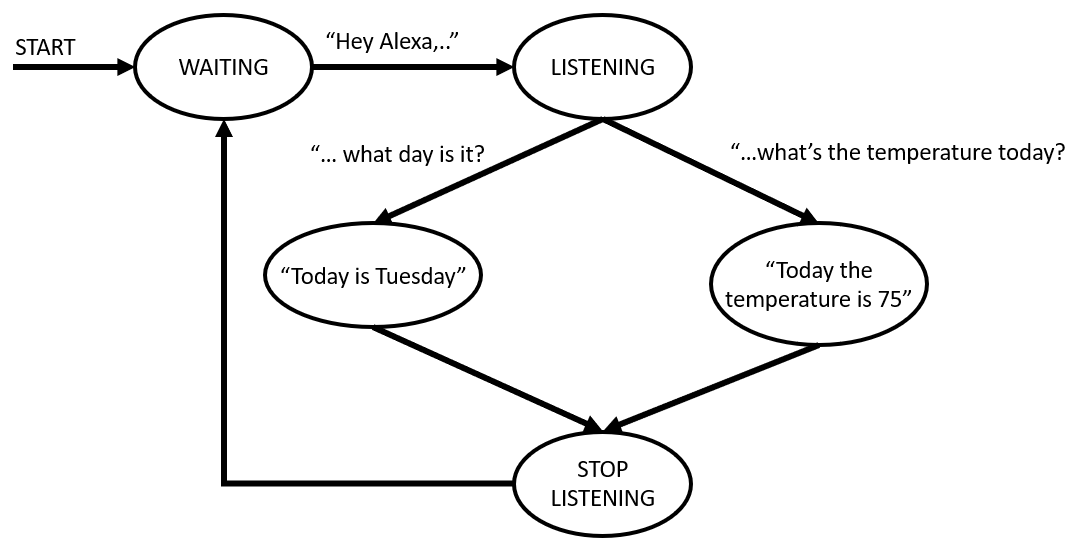
\includegraphics[width=0.9\textwidth]{./figs/alexa.png}
\caption{A simplified state diagram of how an Alexa might be conceptualized. It shows we start in a \textit{WAITING} state, and upon hearing ``Hey Alexa'' we then go to a \textit{LISTENING} state. From there we can listen to multiple commands (in this case just asking for the day of week or temperature), and finally we reach the \textit{STOP LISTENING} state upon which we just return back to the \textit{WAITING} state}
\label{fig:alexa}
\end{figure}

\subsection{Deterministic Finite Automata}
\label{subsect:DFA}
Formally, we can look at state machines to give a complete picture of functionality, and to create a graph of the machine. From wikipedia we can see that there are 5 requirements for a deterministic finite automaton.

\begin{itemize}
\item A finite set of states.
\item A finite set of input symbols.
\item A transition function. This is what defines how we go from one state to another.
\item An initial state.
\item A set of accept states.
\end{itemize}

By looking at the example figure we can break the abstract requirements of a deterministic finite automaton into a concrete form. 

\begin{figure}[!h]
\centering
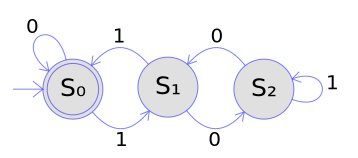
\includegraphics[width=0.9\textwidth]{./figs/DFA.png}
\caption{Sample deterministic finite automaton from wikipedia.}
\label{fig:DFA}
\end{figure}

From Figure \ref{fig:DFA} he finite set of states we can state the following...
\begin{itemize}
\item The finite set of states $Q = \{S_0, S_1, S_2\}$
\item The finite set of input symbols $\Sigma = \{0,1\}$
\item The transition function $\delta$ can be given by the following table that maps the state and input symbol to another state or in other words $\delta = Q \times \Sigma \rightarrow Q$
\begin{center}
\begin{tabular}{|c|c|c|}
\hline 
Current State & Input Symbol & Next State \\ 
\hline 
$S_0$ & $0$ & $S_0$ \\ 
\hline 
$S_0$ & $1$ & $S_1$ \\ 
\hline 
$S_1$ & $0$ & $S_2$ \\ 
\hline 
$S_1$ & $1$ & $S_0$ \\ 
\hline 
$S_2$ & $0$ & $S_1$ \\ 
\hline 
$S_2$ & $1$ & $S_2$ \\ 
\hline 
\end{tabular} 
\end{center}

\item The start state $q_0 = S_0$ which must be some state in our set of states (meaning that $q_0 \in Q$).
\item The set of accept states $F = \{S_0\}$ which is shown in the diagram with the double circle. The accept states must be a subset of all of the states in our DFA (meaning that $F \subseteq Q$)
\end{itemize} 

With these formalized definitions we can analyze performances of applications, and we can also look at if a particular set of inputs will lead us to an output state. For more information go check out NFAs (nondeterministic finite automata) which are a more generalized form of DFAs.

\section{Your task...}
... regardless of whether you choose to accept it is to read in a text file that will contain (in this order)

\begin{enumerate}
\item list of states separated by comma(s)
\item list of inputs separated by comma(s)
\item the starting state
\item list of connections in the form of \begin{verbatim}
currentState,input,nextState
\end{verbatim}
\end{enumerate}

An example of this file would look like the following (based off the example in Section \ref{subsect:DFA}.

\begin{verbatim}
S0,S1,S2
0,1
S0
S0,0,S0
S0,1,S1
S1,0,S2
S1,1,S0
S2,0,S1
S2,1,S2
\end{verbatim}

We can assume that the input we are given will always be in this form and won't have to worry about errors in input like having the same state listed multiple times, or other user errors.

Once read in we should output the current state, and allow the user to input a valid input string, and we will use that to go to the next state. Once at the next state we will output the current state and allow for another input string to be entered. This process will continue until the user enters ``EXIT''. Below is an example session.

\begin{verbatim}
CURRENT STATE: S0
> 0
CURRENT STATE: S0
> 1
CURRENT STATE: S1
> 0
CURRENT STATE: S2
> 0
CURRENT STATE: S1
> EXIT
\end{verbatim}

\subsection{For C}
For solutions in C we will store the data in a much more efficient methodology. Instead of having states and transitions as strings we will handle them as an individual byte (stored in an unsigned char) and will be displayed as a hex value. We can also take some extra steps to improve efficiency and will load the data in the following way (in bytes). The main one to note immediately is that instead of storing strings for the state names or the inputs, we will just assume that all of both will be hex values 0x00-0xFF. So if we have 0x03 states, they will be numbered 0x00-0x02, and if we have 0x10 inputs, they will be 0x00-0x0F.

\begin{enumerate}
\item one byte determining the number of states
\item one byte determining the number of inputs
\item one byte determining the starting state
\item $S \times I$ 2d array of bytes that tell the next state given the current state and input. This is ordered in precedence by starting with state 0x00 and listing all next states given the 0x00-$I$ inputs, then the next state is listed with the next state given all inputs, etc.
\end{enumerate}

A sample input.dat file (again based on the example in Section \ref{subsect:DFA}) is shown below as hex values. The line breaks between bytes are given to help show how the information is broken down.

\begin{verbatim}
03
02
00
00 01
02 00
01 02
\end{verbatim}

For reference in the amount of space saved, the ascii text totaled 73 bytes and our byte storage saved essentially the same information in 9 bytes. The key note here is that we traded functionality (ability for custom state names, custom inputs, more than 255 states, etc) for efficiency (in terms of space, but hopefully in terms of speed as well).

\section{Helpful Notes}
It's a challenging problem at first so take time to make sure that you fully understand the problem. Try making up your own DFA and drawing out the diagram, convert it to the text format, and try stepping through that text file section by section for how you read the data.

You should also take note of what data needs to be accessed when. We don't necessarily need information about all transitions between states at all times, we just need to know the information about the transition for the states we are in. This means the way we store data should allow us to easily access the data we need when we need it.

\section{Additional Features}
For those who would like to really make the most of this exercise there are a few features that could be added.

\begin{itemize}
\item Handle the data file as a command line parameter
\item Handle invalid input strings (alerting the user of their error)
\item Ability to save current state as the new starting state
\end{itemize}

\section{Future Applications}
Beyond diving into more theoretical work, we can take this idea and go towards something more practical (or more fun). Hopefully, you can see that the state machine is a general concept and there are numerous ways to utilize it. Maybe it could be used to keep track of a command line game where you have rooms connected together. 

State machines have a particularly good use in embedded systems that rely on a compact way of storing and accessing functionality as fast as possible. Examples can be anything from a traffic light program, to sensor monitors.

\end{document}